
\section{Optimal control formulation}

In this section, we show the optimal control formulation for selective harmonic elimination for  two-level.

\begin{problem}\label{OCP1}
    Given  a two set of odd numbers $\mathcal{E}_a$ and $\mathcal{E}_b$ with carinalities $|\mathcal{E}_a| = N_a$ and  $|\mathcal{E}_b| = N_b$, given the target vectors $\bm{a}_T  \in \mathbb{R}^{N_a}$ and $\bm{b}_T  \in \mathbb{R}^{N_b}$, we search a wave form $f(\tau ) \ | \ \tau \in (0,\pi)$ which minimimize the follow functional:
        \begin{gather}
        J[f(\tau)] = \Bigg[ || \bm{a}_T - \bm{\alpha}(T)||^2 + || \bm{b}_T - \bm{\beta}(T)||^2 
        + \epsilon \int_0^{\pi} \mathcal{L}[f] d\tau \Bigg] 
    \end{gather}

    where  $\bm{\alpha}(\tau) \in \mathbb{R}^{N_a} \times [0,\pi]$ and $\bm{\beta}(\tau) \in \mathbb{R}^{N_b}  \times [0,\pi]$, the $||.||$ is a euclidean norm and $\epsilon$ is a small parameter to multiple the functional term $\mathcal{L}[f]$. 
    \newline

    In this way, the optimal control problem can be written: 
    \begin{gather}
        \min_{|f(\tau) |<1} J[f(\tau)] \\
        \notag \text{suject to: } \\
        \notag \forall i \in \mathcal{E}_a\ \ 
        \begin{cases}
            \dot{\alpha}_i(\tau) = (2/\pi) \cos(i\tau) f(\tau) & \tau \in [0,\pi]\label{dyn}\\
            \alpha_i(0) = 0
        \end{cases} \\
        \notag \forall j \in \mathcal{E}_b\ \ 
        \begin{cases}
            \dot{\beta}_j(\tau) = (2/\pi) \sin(j\tau) f(\tau) & \tau \in [0,\pi]\label{dyn}\\
            \beta_j(0) = 0
        \end{cases} \\
    \end{gather}
\end{problem}

En el problema de SHE, se busca una función $\{f(\tau) \ |  \tau \in [0,\pi/2] \}$  que solo pueda tomar los valores $\{-1,1\}$. Este tipo de funciones son conocidas en la literatura como controles \emph{bang-bang}. Sin embargo, la solución del problema (\ref{OCP1}) para un término $\mathcal{L}[f]$ general, no tiene porque ser una función \emph{bang-bang}. Con el fin de encontrar las propiedades de $\mathcal{L}[f]$ para que esto suceda escribiremos las condiciones necesarias de optimalidad. 

Entonces siguiendo el principio de mínimo de Pontryagin, escribimos el Hamiltoniano del problema:

\begin{gather}\label{hamil}
    H(f,\bm{p}^\alpha,\bm{p}^\beta,\tau) = \epsilon \mathcal{L}[f] + 
    G(\bm{p}^\alpha,\bm{p}^\beta,\tau) f
\end{gather}

Donde  $G(\bm{p}^\alpha,\bm{p}^\beta)$ es:
    \begin{gather}
        G(\bm{p}^\alpha,\bm{p}^\beta,\tau) = \frac{2}{\pi} \Bigg[ 
            \sum_{i \in \mathcal{E}_a} p^\alpha_i \cos(i\tau)+ 
            \sum_{j \in \mathcal{E}_b} p^\beta_j \sin(j\tau) 
        \Bigg]
    \end{gather}

y además donde $\bm{p}^\alpha \in \mathbb{R}^{N_a} \times [0,\pi]$ y $\bm{p}^\beta \in \mathbb{R}^{N_b}  \times [0,\pi]$ son los estados adjuntos correspondientes a los estados $\bm{\alpha}$ y $\bm{\beta}$ respectivamente. 
\newline 

Utilizando la siguiente condición de optimalidad:
\begin{gather}\label{minH}
    H(\tau,\bm{p}_*^\alpha,\bm{p}^\beta_*,f_*) \leq
    H(\tau,\bm{p}_*^\alpha,\bm{p}^\beta_*,f)
\end{gather}

Podemos obtener la forma del control óptimo cuando los co-estados óptimos $\bm{p}_*^\alpha$ y $\bm{p}_*^\beta$ además de la variable temporal $\tau$ están fijas. 
%
Entonces el problema se reduce la minimización de una función $H^*(f) = H(\tau,\bm{p}_*^\alpha,\bm{p}^\beta_*,f)$ en una variable $f$ dentro de un intervalo $[-1,1]$.
%
Dado que necesitamos que el control óptimo $f^*$ sea \emph{bang-bang}, el mínimo de $H^*(f)$ debe estar en los extremos del intervalo.
En el caso de una variable solo podemos conseguir este comportamiento si no existe ningún mínimo dentro del intervalo. Una manera de asegurar que no existe ningún mínimo dentro del intervalor es tomando la función $H^*(f)$ concava. De esta manera, podemos diseñar la función $H^*(f)$ mediante el término $\mathcal{L}[f]$ ya que derivando dos veces (\ref{hamil}) obtenemos:

\begin{gather}
    \frac{d^2{H^*}^2}{d\tau^2} = \epsilon \frac{d^2\mathcal{L}[f]}{df^2} 
\end{gather}

Es decir la concavidad del término de penalización $\mathcal{L}[f]$ define la concavidad de $H^*(f)$. Así que siempre que elijamos un término de penalización tal que:

\begin{gather}
    \frac{d^2L[f]}{df^2} \leq 0 
\end{gather}

obtendremos control óptimo $f^*$ será \emph{bang-bang}.
\newline

\begin{figure}[!ht]
    \centering
    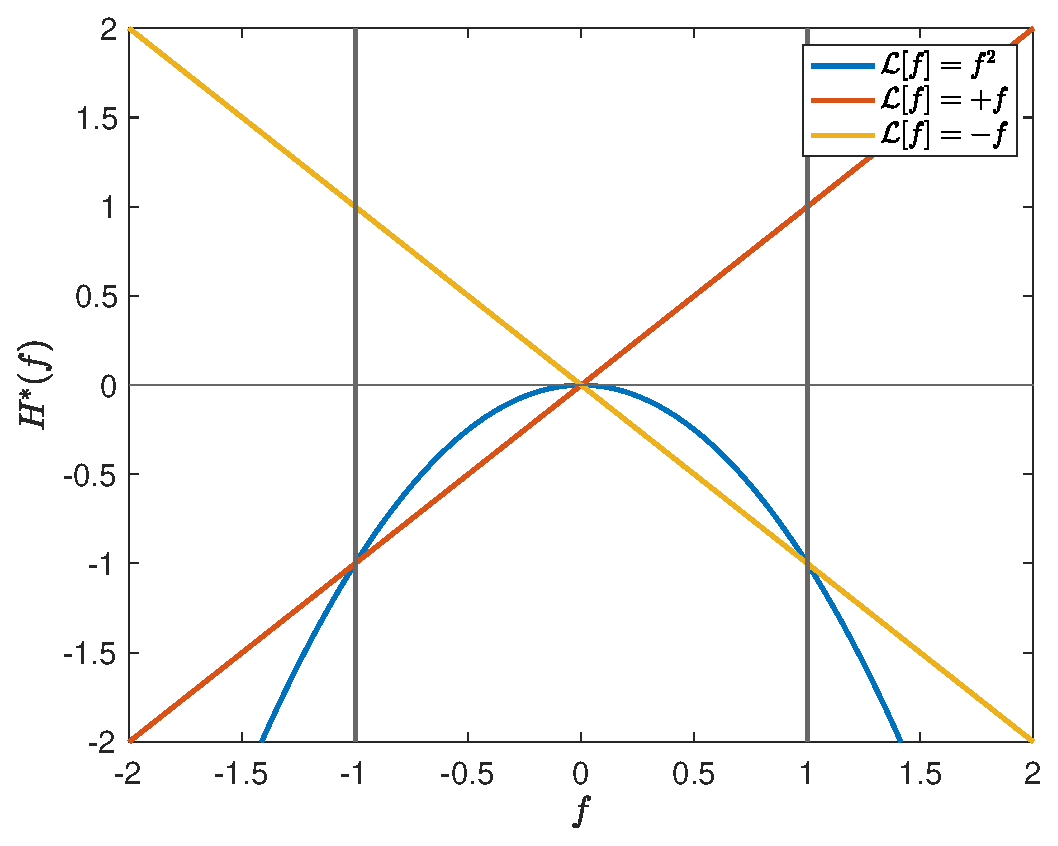
\includegraphics[scale=0.5]{img/bang-bang.eps}
    \caption{Ilustración sobre el comportamiento de la función $H^*(f)$ para distintos términos de penalización $\mathcal{L}[f]$}
\end{figure}


\subsection{OC SHE in two levels for symmetry of quarter-wave} 

Consideraremos un caso concreto del problema presentado en la sección anterior. Este es problema de selective harmonic elimination con simetría de cuarto de onda. Esta simetría implíca:
\begin{gather}
    f(\tau + \pi/2)   = f(\tau)    \ \ \tau \in (0,\pi/2)
\end{gather}

So this condition simplify the expressions of Fourier coefficients (\ref{an}) and (\ref{bn}), in this way:
\begin{align}
    a_i = & \  0 \ \ | \  \ \forall i \in \mathbb{Z} \\
    b_j = &  \frac{4}{\pi} \int_0^{\pi/2} f(\tau ) \sin(j\tau)d\tau \ | \ \forall j \ odd
\end{align}

In summary $f(\tau )$ can be written as follows:
\begin{gather}
    f(\tau ) = \sum_{j \ odd}^\infty  b_n \sin(j \tau) \\
    b_j = \frac{4}{\pi}\int_0^{\pi/2} f(\tau ) \sin(j\tau)d\tau \ \ | \ \ j \ odd \label{bn_odd}
\end{gather}


Now in this context, we can define a SHE problem as follows:


\begin{problem}\label{OCP_bn}
    Given  a set of odd numbers $\mathcal{E}_b$ with carinality $|\mathcal{E}_b| = N_b$ and given the target vector $\bm{b}_T  \in \mathbb{R}^{N_b}$, we search a wave form $f(\tau ) \ | \ \tau \in (0,\pi/2)$ such that $f(\tau)$ that minimize the following functional:

        \begin{gather}
        J[f(\tau)] = \Bigg[ || \bm{b}_T - \bm{\beta}(T)||^2 + \epsilon \int_0^{\pi/2} \mathcal{L}[f(\tau)] d\tau \Bigg] 
    \end{gather}

    where $ \bm{\beta}(\tau) \in \mathbb{R}^{N_b} \times [0,\pi/2] $, the $||.||$ is a euclidean norm and $\epsilon$ is a penalization parameter.
    \newline

    So, the optimal control problem can be written: 
    \begin{gather}
        \min_{|f(\tau) |<1} J[f(\tau)] \\
        \notag \text{suject to: } \\
        \notag \forall j \in \mathcal{E}_b \
        \begin{cases}
            \dot{\beta_j}(\tau) = (4/\pi) \sin(j\tau) f(\tau) & \tau \in [0,\pi/2]\label{dyn}\\
            \beta_j(0) = 0
        \end{cases} 
    \end{gather}
\end{problem}

En este caso el problema de control tiene el siguiente Hamiltoniano:
\begin{gather}
    H(f,\bm{p}_\beta,\tau) = -\epsilon  \mathcal{L}[f]+ 
    \frac{4f}{\pi} \Bigg[ 
        \sum_{j \in \mathcal{E}_b} p^\beta_j \sin(j\tau) 
    \Bigg]
\end{gather}

Podemos ver que el Hamiltoniano tiene la misma estructura que en el caso anterior, por lo que de la misma forma la elección de un término de penalización $\mathcal{L}[f]$ concavo nos produce un control óptimo $f^*$ \emph{bang-bang}.
